% !TeX spellcheck = en_US
\chapter{Implementation}%
\label{sec:implementation}

A MATLAB\textsuperscript{\textregistered} Simulink~\cite{MATLAB:2022} implementation of the JenaFox model, reflecting the test environment described in the upcoming section~\ref{sec:jenafox}, was provided. A modified neural network controller based on the work of~\citeauthor{Geng2006}~\cite{Geng2006} was used as a controller, which is discussed in more detail in section~\ref{sec:neural-controller}. The concept of~\glsxtrfull{vlo}, proposed by~\citeauthor*{Rummel2010}~\cite{Rummel2010} and described in section~\ref{sec:vlo}, was taken as initial and final condition,~\ie one iteration of the simulation consists of one full step or one half of a stride, respectively. The iterations were finally analyzed using a trajectory optimization, described in section~\ref{sec:trajectory-optimization}, in order to achieve a solution that is as periodic as possible, in other words, with as little difference as possible between the final and initial conditions of the robot.

% !TeX spellcheck = en_US
\section{The JenaFox Bipedal Walking Robot}
\label{sec:jenafox}

    JenaFox refers to a bipedal robot developed at the Friedrich-Schiller-University Jena in Germany, designed for research in robotics and control engineering with a focus on bipedal locomotion. The robot resembles two human-like legs, connected by a torso, that are capable of walking and navigating different terrains. The system is equipped with a variety of sensors, such as accelerometers and gyroscopes, which provide data on its motion and orientation. This data can then be used to control the robot's actuators and thus its movements, allowing it to balance, walk, and respond to its environment in real-time. The robot is also designed to be highly scalable and modular, with a wide range of interchangeable components that can be customized to meet specific research needs. This includes the ability to easily swap out different sensors, actuators, and control boards, allowing researchers to easily experiment with different configurations and components.~\cite{Renjewski2012}\\

    The robotic test environment is unique in that it is designed as an open-source platform, making it accessible to researchers and students who want to study and experiment with bipedal robotics. Overall, JenaFox is a valuable tool for researchers and students in the field of robotics and control engineering, as it provides a platform for exploring the challenges and opportunities associated with bipedal locomotion, and for developing new technologies and control strategies for robots.~\cite{Renjewski2012}\\

    A schematic representation of the JenaFox robot is shown in figure~\ref{fig:jenafox-wireframe}. The bipedal robot consists of a torso connected to two segmented legs, each of which has an upper and a lower link. When taking a step, the stance leg supports the weight of the robot, while the swing leg is free to move above the ground. All limbs are connected via actuators, with sensors in each joint measuring angular position and velocity, except for the ankle joint, which is the only passive joint of the system. The trunk of the robot is attached to a boom via a freely rotating joint. The tether mechanism constrains the motion of the robot on a sphere, without excessively affecting its dynamics in the sagittal plane (\ie the plane spanned between the abscissa axis (X-axis, orange) and ordinate axis (Y-axis, green), see figure~\ref{fig:coordinate-system}). The mechanism consists of an aluminum tube, a spherical pivot fixed to the floor and a tension cable. The tether is instrumented to provide measurements of the machine's three motions: vertical translation, forward translation, and rotation about the axis of the boom.~\cite{Renjewski2012}~\cite{Renjewski2013}

    \begin{figure}[htb]%
        \centering%
        \begin{subfigure}{0.5\linewidth}%
            \centering%
            
\includegraphics[width=0.8\linewidth]{jenafox/jenafox-wireframe-transparent-black-thick.png}
            \caption{Schematic representation of the JenaFox robot. (Adapted from~\cite{Jenafox:Wireframe})}%
            \label{fig:jenafox-wireframe}%
            %
        \end{subfigure}%
        %
        \hfil%
        %
        \begin{subfigure}{0.5\linewidth}%
            \centering%
            \includestandalone{coordinate-system/coordinate-system}%
            \caption{Definition of the associated coordinate system.\newline}%
            \label{fig:coordinate-system}%
            %
        \end{subfigure}%
        %
        \caption{Schematic representation of the JenaFox bipedal walking robot (\subref{fig:jenafox-wireframe}) with its associated coordinate system (\subref{fig:coordinate-system}). The bipedal robot consists of a torso connected to two segmented legs, each of which has an upper and a lower link. The abscissa axis (X-axis, orange) points in the direction of motion, the ordinate axis (Y-axis, green) points upward. The trunk of the robot is attached to a boom via a freely rotating joint which constrains the motion of the robot on a sphere. The planar motion is thus restricted to the sagittal plane (\ie the plane spanned between the abscissa axis and ordinate axis).}%
        \label{fig:jenafox}%
    \end{figure}
    % \noindent
    %
    The simulation of the JenaFox robot is created in MATLAB\textsuperscript{\textregistered} Simulink R2022a as a Simscape multi-body model. The solver settings used for the simulation are listed in table~\ref{tab:solver-settings}.

    \begin{table}[H]
        \caption{Solver settings for the MATLAB\textsuperscript{\textregistered} Simulink simulation of the JenaFox robot.} 
        \label{tab:solver-settings}
        \begin{center}
            \begin{tabular}{ l|l }
                \textbf{Solver setting} & \textbf{Value}                \\ [0.5ex]
                \hline \hline
                Solver type             & variable-step                 \\
                Solver                  & auto(\glsxtrshort{ode}15s)    \\ % \glsxtrshort{ode}23s (Min./ Rosenbrock) \\
                Max step size           & 0.1                           \\
                Min step size           & auto                          \\
                Relative tolerance      & 0.01                          \\
                Absolute tolerance      & 0.001                         \\
            \end{tabular}
        \end{center}
    \end{table}
    %
%
% !TeX spellcheck = en_US
\section{Neural Network Controller}
\label{sec:neural-controller}

    In the simulation, a neural network controller based on the work of~\citeauthor{Geng2006}~\cite{Geng2006} is used. The authors propose that a bio-inspired neural network controller may perform better in biped control than other comparable solution methods, such as zero moment point or~\glsxtrlong{ip} control, as it guarantees a stable gait even at high speeds. A neural network controller is a type of artificial intelligence algorithm that uses the principles of artificial neural networks to control the behavior of a system. Neural networks are modeled after the structure and function of the human brain, and they are trained using large amounts of data to learn how to perform a particular task. In the context of a neural network controller, the network is trained to produce control signals for a system based on inputs that represent the state of the system. These inputs could include sensor readings, past control signals, or other relevant information about the system. The neural network then outputs control signals that are used to regulate the behavior of the system. One of the key benefits of using a neural network controller is that, despite being highly scalable and flexible, it can learn to perform complex tasks that are difficult to describe mathematically. For example, a neural network controller could be trained to control a robot to walk, swim, or fly in a way that is similar to how animals perform these tasks. The network can learn from examples and adapt to new situations, making it well-suited for tasks that are subject to unpredictable variations or changing conditions.~\cite{Geng2006}\\

    Despite its many benefits, there are also some challenges associated with using a neural network controller. One of these challenges is that it can be difficult to interpret how the network is making decisions, since the internal workings of the network are often highly complex and non-linear. Identifying and correcting errors in the network's behavior is therefore a demanding task. Another challenge is that neural networks are often trained using large amounts of data. The downside of this approach is its intensive and time-consuming computation. Therefore it is difficult to use neural network controllers in real-time applications, where the control signals need to be generated quickly and with a high level of accuracy.~\cite{Geng2006}\\
    
    Table~\ref{tab:control-scheme} gives an overview of the control scheme used for the JenaFox robot. Touchdown and reaching the~\glsxtrfull{aea} of either hip angle triggers the corresponding action. When the target is reached the power of the moving motors is switched off. Thus, the phases of the gait are:

    \begin{enumerate}
        \item Until the moment of touchdown, the right knee is extended while the right hip is flexed.
        \item As soon as the double support phase is reached, the right hip begins to extend while the left knee flexes, thus leaving the ground. The double support phase is relatively short.
        \item When the left knee is fully bent, the left hip begins to flex while the right hip continues to extend. The left leg thus surpasses the right and is now in front.
        \item When the left hip reaches the~\glsxtrshort{aea}, the left knee begins to extend. The right hip remains extended.
        \item Before touchdown, the right hip and the left knee are extended to their limits.
    \end{enumerate}

    \begin{table}[H]
        \caption{Overview of the control scheme used for the JenaFox robot. Touchdown (TD) and reaching the~\glsxtrfull{aea} of either hip angle triggers the corresponding action. When the target is reached the power of the moving motors is switched off. In the images, the events are shown as dark stick figures and the corresponding actions as light stick figures. (Adapted from~\cite{Renjewski2013}, p. 36)} \label{tab:control-scheme}
        \begin{center}
            \begin{tabular}{ l|l r|l r|l r|l r }
                \multicolumn{1}{c|}{\textbf{Event}}                   &
                \multicolumn{2}{c|}{\textbf{1. TD\textsubscript{r}}}  &
                \multicolumn{2}{c|}{\textbf{2. HL@\glsxtrshort{aea}}} &
                \multicolumn{2}{c|}{\textbf{3. TD\textsubscript{l}}}  &
                \multicolumn{2}{c}{\textbf{4. HR@\glsxtrshort{aea}}}  \\ 
                \hline \hline
                & \textit{action} & \textit{goal} & \textit{action} & \textit{goal} & \textit{action} & \textit{goal} & \textit{action} & \textit{goal} \\
                left hip (HL) & flex & \glsxtrshort{aea} & & & extend & \glsxtrshort{pea} & & \\
                left knee (KL) & flex & \glsxtrshort{pea} & extend & \glsxtrshort{aea} & hold & \glsxtrshort{aea} & & \\
                right hip (HR) & extend & \glsxtrshort{pea} & & & & flex & \glsxtrshort{aea} \\
                right knee (KR) & hold & \glsxtrshort{aea} & & & flex & \glsxtrshort{pea} & extend & \glsxtrshort{aea} \\
                \hline
                & \multicolumn{2}{c|}{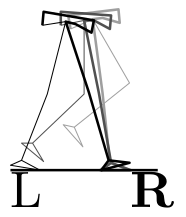
\includegraphics[width=0.1\textwidth]{control-scheme/TD-r.png}} & \multicolumn{2}{c|}{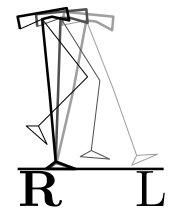
\includegraphics[width=0.1\textwidth]{control-scheme/Hip-l.png}} & \multicolumn{2}{c|}{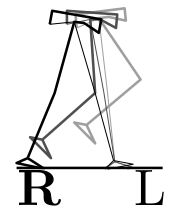
\includegraphics[width=0.1\textwidth]{control-scheme/TD-l.png}} & \multicolumn{2}{c}{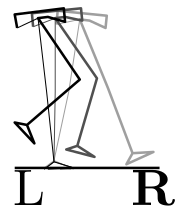
\includegraphics[width=0.1\textwidth]{control-scheme/Hip-r.png}} \\
            \end{tabular}
        \end{center}
    \end{table}

    Figure~\ref{fig:jenafox-ISB-convention} shows the control parameters used for the joint angles according to the~\glsxtrfull{isb}\footnote{The~\glsxtrshort{isb} is a non-profit organization founded in 1973 dedicated to promoting the study and application of biomechanics around the world.} convention~\cite{Jenafox:ISB}. The parameter set consists of eight angles and five voltage values,~\ie for both the left and right leg two extreme angles each for hip and knee with respective voltage values for extension and flexion of each joint. The fifth voltage value represents the hold voltage of the knee in stance to keep the leg straight.~\cite{Renjewski2013}

    \begin{figure}[H]% 
        \centering%
        \begin{subfigure}{0.5\linewidth}%
            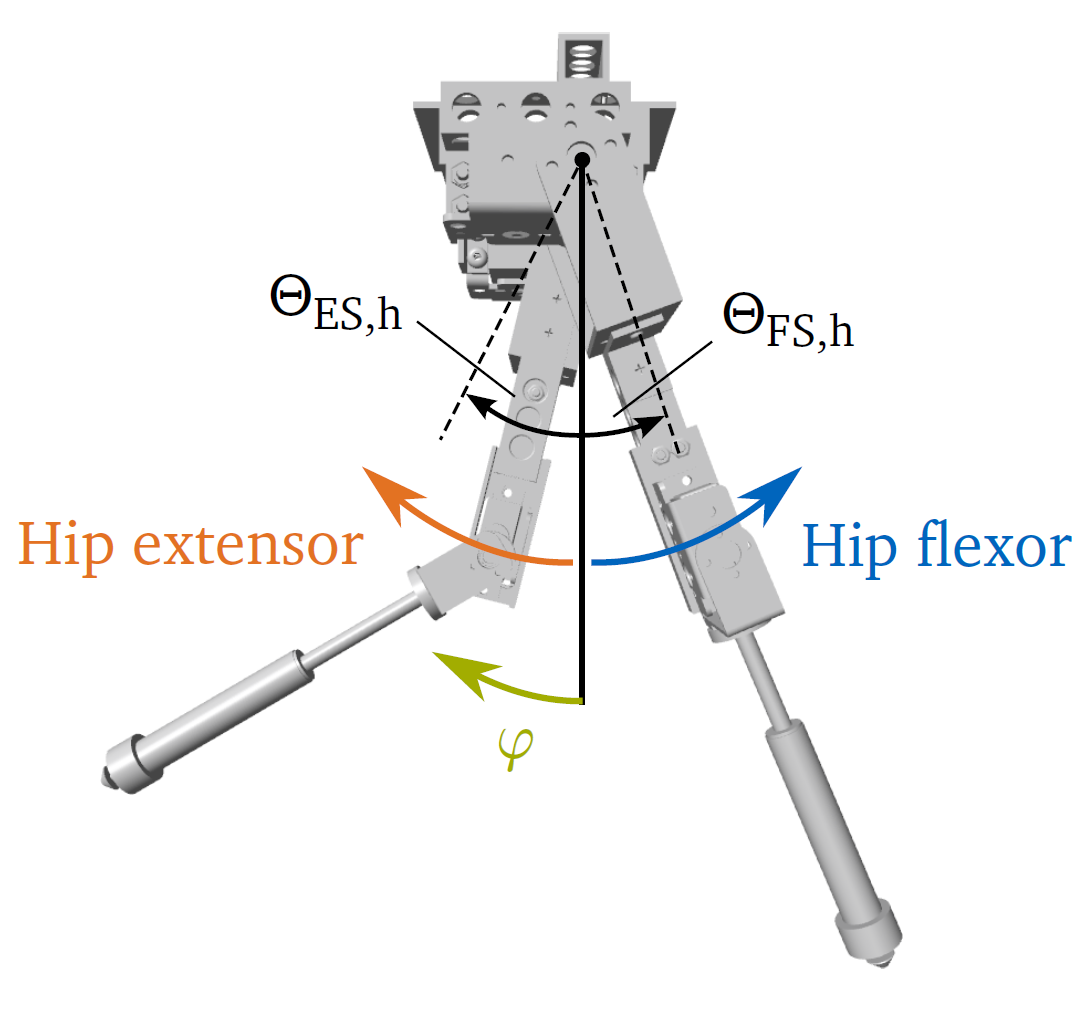
\includegraphics[width=\linewidth]{jenafox/jenafox-ISB-convention-hip.png}
            \caption{Control parameters for the hip joints.}
            \label{fig:jenafox-ISB-convention-hip}%
        \end{subfigure}%
        %
        \hfil%
        %
        \begin{subfigure}{0.5\linewidth}%
            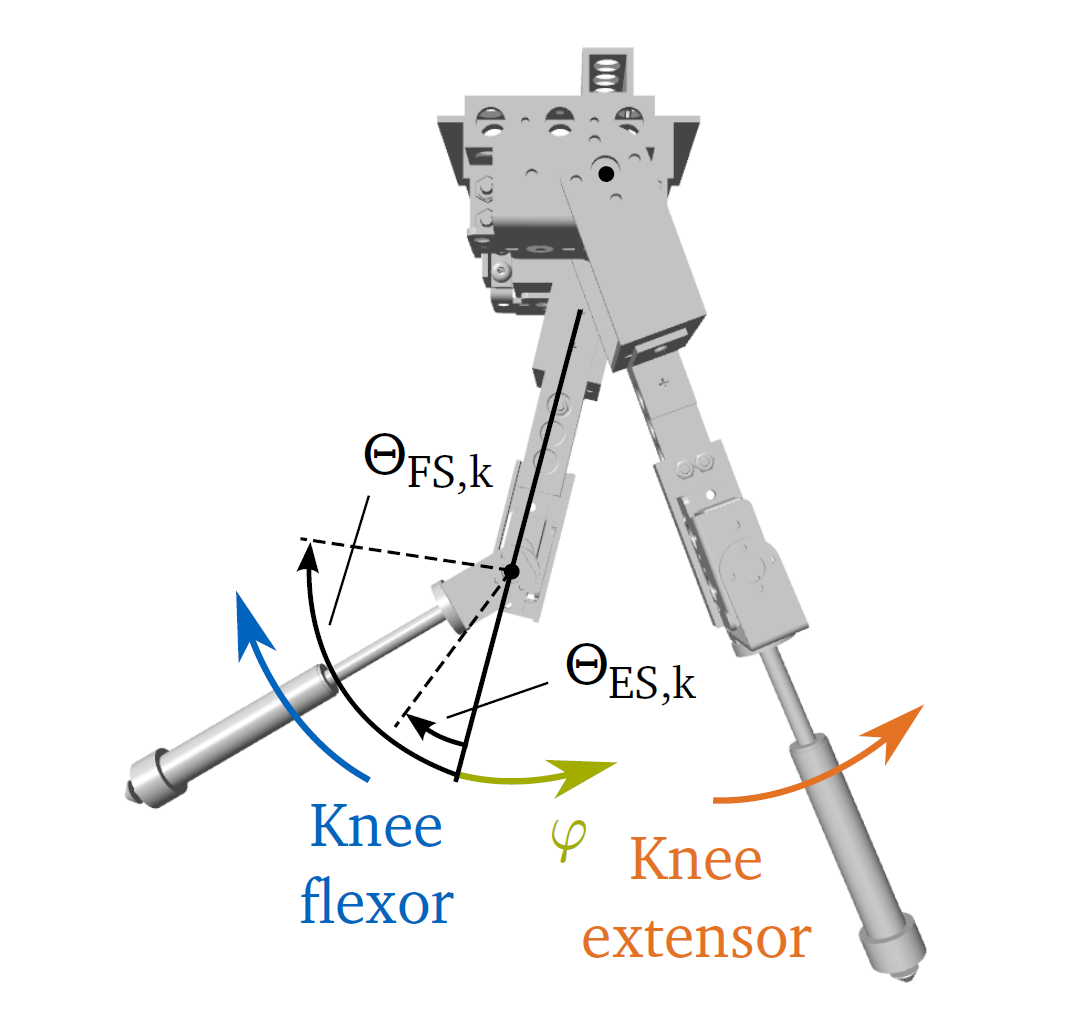
\includegraphics[width=\linewidth]{jenafox/jenafox-ISB-convention-knee.png}
            \caption{Control parameters for the knee joints.}
            \label{fig:jenafox-ISB-convention-knee}%
        \end{subfigure}%
        %
        \caption{The control parameters for the hip (\subref{fig:jenafox-ISB-convention-hip}) extensor $\gls{theta-es}_{,h}$ (orange) and flexor $\gls{theta-fs}_{,h}$ (blue) as well as the knee (\subref{fig:jenafox-ISB-convention-knee}) extensor $\gls{theta-es}_{,k}$ (orange) and flexor $\gls{theta-fs}_{,k}$ (blue) joint angles according to the~\glsxtrlong{isb} convention. (Adapted from~\cite{Jenafox:ISB})}%
        \label{fig:jenafox-ISB-convention}%
    \end{figure}%
    % \noindent
    
    The~\glsxtrshort{aea} is obtained by mapping the angle of the projected velocity vector,~\ie the velocity vector of the~\glsxtrshort{com}$~\gls{v}_{\glsxtrshort{com}}$ projected down to the hip with a mapping function. The projected velocity vector$~\gls{v}_{CH}$ is calculated as the cross product of the angular velocity of the~\glsxtrshort{com} $\dot{\phi}_{\glsxtrshort{com}}$ with the vector from the hip to the~\glsxtrshort{com} summed with the translational velocity of the~\glsxtrshort{com}:

    \begin{align}
        \gls{v}_{CH} &= 
            \begin{bmatrix}
                \gls{v}_{CH_x}  \\
                \gls{v}_{CH_y}  \\
                0 \\
            \end{bmatrix} = 
            \begin{bmatrix}
                \gls{v}_{\glsxtrshort{com}_x}  \\
                \gls{v}_{\glsxtrshort{com}_y}  \\
                0 \\
            \end{bmatrix} + \left(
            \begin{bmatrix}
                0   \\
                0   \\
                \dot{\phi}_{\glsxtrshort{com}} \\
            \end{bmatrix} \times
            \begin{bmatrix}
               x_{hip} - x_{\glsxtrshort{com}}   \\
               \gls{y}_{hip} - \gls{y}_{\glsxtrshort{com}}   \\
               0         \\
            \end{bmatrix}
            \right).
    \end{align}
    % \noindent
    
    The corresponding angle$~\gls{rho}$ is obtained by

    \begin{align}
        \gls{rho} &= \textrm{arctan2}\left( \frac{\gls{v}_{CH_y}}{\gls{v}_{CH_x}} \right)
    \end{align}
    % \noindent

    where $\textrm{arctan2}$ is the four-quadrant inverse tangent, returning values in the closed interval $\left[-\pi, \pi\right]$, as shown in figure~\ref{fig:atan2}. Note that$~\gls{rho}$ and the~\glsxtrshort{aea} are oriented in opposite directions, as shown in figure~\ref{fig:lambda-aea}. \\

    \begin{figure}[htb]% 
        \centering%
        \begin{subfigure}{0.5\linewidth}%
            \centering%
            \includestandalone{atan2/atan2}
            \caption{The four-quadrant inverse tangent.}
            \label{fig:atan2}
        \end{subfigure}%
        %
        \hfil%
        %
        \begin{subfigure}{0.5\linewidth}%
            \includestandalone{lambda-aea/lambda-aea}
            \caption{Alignment of$~\gls{rho}$ (blue) and the~\glsxtrshort{aea} (green).}
            \label{fig:lambda-aea}
        \end{subfigure}%
        %
        \caption{Graphical representation of the four-quadrant inverse tangent, returning values in the closed interval $\left[-\pi, \pi\right]$ (\subref{fig:atan2}) and alignment of$~\gls{rho}$, the angle of the projected velocity vector$~\gls{v}_{CH}$ (blue), and the~\glsxtrfull{aea} (green). Note that the angles are oriented opposite to each other (\subref{fig:lambda-aea}).}%
        \label{fig:lambda-proj}%
    \end{figure}%
    % \noindent
    
    In order to achieve an adequate mapping from$~\gls{rho}$ to the~\glsxtrshort{aea}, various mapping functions were tested. The first set of experiments tested linear functions that set the~\glsxtrshort{aea} in direct proportional dependence to$~\gls{rho}$, with the desired effect that the steeper$~\gls{rho}$ becomes, the steeper should also the~\glsxtrshort{aea} become to consequently obtain a steeper angle of attack~\gls{alpha} and thus exchange as much vertical for horizontal velocity as possible. A selection of linear functions used is given in the following figure~\ref{fig:linear-mapping}. However, it quickly became apparent that a linear mapping function is not optimal in many ways, since these tend to quickly leave the interval of reasonable values of the~\glsxtrshort{aea}. Thus, the next step was to try to achieve a better mapping via exponential functions, which are shown in figure~\ref{fig:exponential-mapping}. One problem with exponential mapping functions is that there only needs to be a very small change in$~\gls{rho}$ to cause a large change in the~\glsxtrshort{aea}. Thus, a sigmoid\footnote{The sigmoid function is a mathematical function known for its characteristic "S"-shaped sigmoid curve and commonly used in machine learning and neural networks, where it can be used as a type of activation function that maps any real-valued number to a value between 0 and 1, which makes it useful for modeling probabilities and binary classification problems.} function was used to map the values of$~\gls{rho}$ to obtain values of the~\glsxtrshort{aea} in a range between $-10\,\textrm{\si{\degree}}$ and $-25\,\textrm{\si{\degree}}$. Mapping$~\gls{rho}$ with the following sigmoid function yields the~\glsxtrshort{aea}:

    \begin{align}
        \text{\glsxtrshort{aea}} &= \frac{15}{1 + e^{\gls{k} \cdot \gls{rho} + \gls{d}}} - 25
        \label{eq:aea}%
    \end{align}
    % \noindent

    where~\gls{k} depicts a proportionality constant and~\gls{d} is an offset,~\ie a shift of the function along the abscissa axis. Values of$~\gls{k} = 0.2$ and$~\gls{d} = 4$ were chosen to map the values of$~\gls{rho}$ to obtain according values of the~\glsxtrshort{aea} in a range between $-10\,\textrm{\si{\degree}}$ and $-25\,\textrm{\si{\degree}}$, as shown in figure~\ref{fig:sigmoid-mapping}. A summary of the control parameters is given in table~\ref{tab:control-parameters-sensory} and table~\ref{tab:control-parameters-motor}.
    
    \begin{figure}[htb]%
        \centering%
        \includestandalone{mapping/linear/linear}
        \caption{Linear mapping functions that set the~\glsxtrfull{aea} in direct proportional dependence to$~\gls{rho}$.}
        \label{fig:linear-mapping}
    \end{figure}%
    % \noindent
    
    \begin{figure}[htb]%
        \centering%
        \includestandalone{mapping/exponential/exponential}
        \caption{Exponential mapping functions that set the~\glsxtrfull{aea} in exponential dependence to$~\gls{rho}$.}
        \label{fig:exponential-mapping}
    \end{figure}%
    % \noindent
    
    \begin{figure}[H]%
        \centering%
        \includestandalone{mapping/sigmoid/sigmoid}
        \caption{Sigmoid mapping functions and graphical representation of equation~\ref{eq:aea}. The sigmoid function maps the projected velocity vector$~\gls{rho}$ to obtain the~\glsxtrfull{aea} in a range between $-10\,\textrm{\si{\degree}}$ and $-25\,\textrm{\si{\degree}}$.}
        \label{fig:sigmoid-mapping}
    \end{figure}%
    % \noindent

    \begin{table}[H]
        \caption{Overview of the used control parameters for the sensory neurons,~\ie the joint angles of the hip extensor$~\gls{theta-es}_{,~h}$ and flexor$~\gls{theta-fs}_{,~h}$ as well as the knee extensor$~\gls{theta-es}_{,~k}$ and flexor$~\gls{theta-fs}_{,~k}$.} 
        \label{tab:control-parameters-sensory}
        \begin{center}
            \begin{tabular}{ l|l|l|l }
                \textbf{Control parameters for sensory neurons}         & \textbf{Description}          & \textbf{Value}        & \textbf{Unit}                 \\ [0.5ex]
                \hline \hline
                $\gls{theta-es}_{,~h}$                                  & Threshold for hip extensor    & $5$                   & $\left[\si{\degree}\right]$   \\
                $\gls{theta-fs}_{,~h}$                                  & Threshold for hip flexor      & \glsxtrshort{aea}     & $\left[\si{\degree}\right]$   \\
                $\gls{theta-es}_{,~k}$                                  & Threshold for knee extensor   & $-5$ - $-3$           & $\left[\si{\degree}\right]$   \\
                $\gls{theta-fs}_{,~k}$                                  & Threshold for knee flexor     & $-80$                 & $\left[\si{\degree}\right]$   \\
            \end{tabular}
        \end{center}
    \end{table}
    
    \begin{table}[H]
        \caption{Overview of the used control parameters for the motor neurons. $\gls{tau}$ is a time constant associated with the passive properties of the cell membrane, $\gls{M-amp}$ represents the magnitude of the servo amplifier. $\gls{GM}_h$ and $\gls{GM}_k$ depict the gain of the hip and knee motor, respectively.} 
        \label{tab:control-parameters-motor}
        \begin{center}
            \begin{tabular}{ l|l|l|l }
                \textbf{Control parameters for motor neurons} & \textbf{Description} & \textbf{Value} & \textbf{Unit} \\ [0.5ex]
                \hline \hline
                $\gls{tau}$     & Time constant                     & $0.01$                    & $\left[\si{\second}\right]$   \\
                $\gls{M-amp}$   & Magnitude of the servo amplifier  &   $3$                     & $-$                           \\
                $\gls{GM}_h$    & Gain of the hip motor             & $1.4$ - $1.8$             & $-$                           \\
                $\gls{GM}_k$    & Gain of the knee motor            & $0.9 \cdot \gls{GM}_h$    & $-$                           \\
            \end{tabular}
        \end{center}
    \end{table}

    $\gls{tau}$ is a time constant associated with the passive properties of the cell membrane~\cite{Gallagher1996} and $\gls{M-amp}$ represents the magnitude of the servo amplifier~\cite{Geng2006}. In the course of this work, the gain of the hip motor$~\gls{GM}_h$ was modulated in the range between 1.4 and 1.8 in steps of 0.1. Furthermore, the threshold for the knee extensor$~\gls{theta-es}_{,~k}$ was modulated in the range between $-5\,\textrm{\si{\degree}}$ and $-3\,\textrm{\si{\degree}}$ in steps of 0.25. The best results were obtained with$~\gls{GM}_h = 1.6$ and$~\gls{theta-es}_{,~k} = -4.25\,\textrm{\si{\degree}}$. The initial velocities of the~\glsxtrshort{com} were set via the following equations:

    \begin{align}
        \gls{v}_{\glsxtrshort{com}_x,~IC} &= \vert \gls{v}_{\glsxtrshort{com}} \vert \cdot \textrm{cos}(\gls{lambda}) \notag \\
        \gls{v}_{\glsxtrshort{com}_y,~IC} &= \vert \gls{v}_{\glsxtrshort{com}} \vert \cdot \textrm{sin}(\gls{lambda})
        \label{eq:com-velocities}%
    \end{align}
    % \noindent

    where $\vert \gls{v}_{\glsxtrshort{com}} \vert$ is the magnitude and$~\gls{lambda}$ the angle of the velocity vector of the~\glsxtrshort{com}. 
    
    % The magnitude of the vector was set depending on$~\gls{GM}_h$ as follows

    % \begin{align}
    %     \vert \gls{v}_{\glsxtrshort{com}} \vert &=~\gls{k} \cdot~\gls{GM}_h
    %     \label{eq:com-velocity-magnitude}%
    % \end{align}
    % % \noindent

    % where~\gls{k} depicts a proportionality constant. Both~\gls{k} and the angle$~\gls{lambda}$ were passed to the optimizer to obtain optimal initial conditions.
    
    % Which are graphically shown in figure~\ref{fig:com-velocities}

    % \begin{figure}[htb]%
    %     \centering%
    %     \includestandalone{com-velocities/com-velocities}
    %     \caption{Graphical representation of equation~\ref{eq:aea}. The sigmoid function maps the projected velocity vector$~\gls{rho}$ to obtain the~\glsxtrfull{aea}.}
    %     \label{fig:com-velocities}
    % \end{figure}%
    % % \noindent
    
%
% !TeX spellcheck = en_US
\section{Vertical Leg Orientation}
\label{sec:vlo}

    The~\glsxtrfull{vlo} refers to the orientation of the leg of a bipedal robot relative to the ground and is defined as the angle between the ordinate axis (perpendicular to the ground) and the line connecting the foot and hip joint of the robot. In a normal walking gait, the~\glsxtrshort{vlo} changes throughout the stride cycle as the robot moves from one foot to the other. During the stance phase, the~\glsxtrshort{vlo} starts at a relatively small angle, increases as the robot transfers weight over the stance leg, and reaches its maximum value just before the swing phase. During the swing phase, the~\glsxtrshort{vlo} decreases as the swing leg moves forward, reaches its minimum value just before the footstrike, and then increases again as the swing leg moves into the stance phase.~\cite{Rummel2010}\\
    
    The JenaFox robot is capable of periodic gait patterns such as walking and running, where a gait pattern is fully described by the system parameters and initial conditions. In the course of this work, the initial conditions are chosen so that the stance leg is in contact with the ground and vertically oriented, \ie the~\glsxtrshort{com} is exactly above the foot point ($\gls{x}_{\glsxtrshort{com}} = \gls{x}_{FP_1}$), meaning that the horizontal position is zero with respect to the actual foot point. A single step is completed when the swing leg attains ground contact and the~\glsxtrshort{com} is orthogonally above the second foot point ($\gls{x}_{\glsxtrshort{com}} = \gls{x}_{FP_2}$), as shown in figure~\ref{fig:vlo}. The simulation starts at the moment of~\glsxtrlong{vlo} during single support phase (\glsxtrshort{vlo}$_0$) and ends after one step is completed at~\glsxtrshort{vlo} of the opposite leg (\glsxtrshort{vlo}$_1$). These initial conditions can be used to reduce the number of independent initial conditions.~\cite{Rummel2010}

    \begin{figure}[htb]%
        \centering%
        \includestandalone{vlo/vlo}
        \caption{The bipedal spring mass model for walking. The simulation starts at the moment of~\glsxtrfull{vlo} during single support phase (\glsxtrshort{vlo}$_0$, green) and ends after one step is completed at~\glsxtrshort{vlo} of the opposite leg (\glsxtrshort{vlo}$_1$, green). The phase of the double support is shown in blue. The trajectory of the~\glsxtrlong{com} is drawn in orange. (Adapted from~\cite{Rummel2010}, p. 1)}%
        \label{fig:vlo}%
    \end{figure}%
    % \noindent
    %

    % \textcolor{red}{In order to identify periodic walking gaits we introduce a Poincare section at the instant of~\glsxtrfull{vlo} during single support (figure~\ref{fig:vlo}), that allows for the investigation of both, walking and running, with the same method. A legged system can be investigated by analyses of single-step Poincare maps of the state vector $S$ with~\glsxtrshort{vlo} as Poincare section. The mapping function is $S_{i+1} = F(S_i)$ where $i$ is the number of the individual step. $S_i$ denotes the system's state at the instant of~\glsxtrshort{vlo} with $S_i = [\gls{y}_i, \theta_i]^T$. A periodic gait pattern (limit-cycle trajectory) corresponds to a fixed point in the Poincare map $S* = F(S*)$. Stability of a periodic solution is estimated by calculating the effect of small perturbations in the neighborhood of the fixed point. Therefore, a linear approximation is applied \left[S_{i+1} - S*] = J(S*)[S_i - S*]$ where $J(S*)$ is the Jacobian matrix, with the eigenvalues $\lambda_j$ called Floquet multipliers. Dynamic stability of the periodic gait s indicated if the magnitude of all eigenvalues is smaller than one (Guckenheimer, 1983).}%
% !TeX spellcheck = en_US
\section{Trajectory Optimization}
\label{sec:trajectory-optimization}

    Trajectory optimization is a method for designing the motion of a system to achieve a desired goal. It involves the calculation of an optimal path taking  various constraints and objectives into account. The term trajectory refers to the path an agent travels as a function of time. The term trajectory optimization is therefore the set of methods used to obtain the best trajectory, usually by selecting appropriate inputs to the system,~\ie controls, as functions of time. The comprehensive policy of optimization is to minimize the objective function subject to a number of constraints and restrictions.~\cite{Kelly2017} In the course of this work a trajectory optimization was performed via finding a minimum of constrained nonlinear multivariable functions.\\ % Therefore, the comprehensive policy is to minimize the objective function subject to the system dynamics and constraints.

    The process typically involves the following steps~\cite{Kelly2017}:
    \begin{enumerate}
        \item Modeling the robot's dynamics: A mathematical model of the robot's movement is created, which takes into account the robot's kinematics, dynamics, and control inputs.
        \item Specifying the constraints: The constraints that must be satisfied by the robot's motion are defined, such as bounds on the joint angles and torques, as well as collision avoidance constraints.
        \item Defining the objective: The objective function to be optimized is defined, which might include a trade-off between energy efficiency, speed, and smoothness of the motion.
        \item Solving the optimization problem: An optimization algorithm is applied to find the path that minimizes the objective function while satisfying the constraints.
        \item Generating the motion trajectory: The optimal path is transformed into a set of points that define the motion trajectory for the robot.
    \end{enumerate}
    
    The following sections describe the individual steps that were carried out in more detail.

        \subsection*{Assumptions}
        
        Within this work it is assumed that the trajectory is single-phase and of continuous time, meaning the system dynamics are continuous throughout the entire trajectory. The dynamics, the objective, and the constraints are smooth, consistent and potentially non-linear. Furthermore, the robot is considered to be left-right symmetric, allowing to search for a periodic walking gait with a single step instead of a stride. A periodic gait requires that the joint trajectories, consisting of the joint angles, their rates, and the associated torques, are the same for each successive step.~\cite{Kelly2017}
        
        \subsection*{Constraints}
        
        % The optimization problem is subject to a number of constraints and restrictions. 
        The first and possibly most important constraint is the system dynamics. In addition, limits are defined for the boundary condition, restricting the initial and final states of the system, including upper and lower limits for the joint angles and joint velocities. Furthermore, the initial state is limited to the~\glsxtrshort{vlo}$_0$,~\ie the stance leg always starts vertically. % Further path constraints were used to keep the foot of the robot above the ground, for example
        
        % The optimization is subject to a variety of limits and constraints. The first, and perhaps most important, of these constraints is the system dynamics. Next is the path constraint, which enforces restrictions along the trajectory. A path constraint could be used, for example, to keep the foot of a walking robot above the ground during a step. Another important type of constraint is a nonlinear boundary constraint, which puts restrictions on the initial and final states of the system. Such a constraint would be used, for example, to ensure that the gait of a walking robot is periodic.
        
        % \subsection{Transcription}

        %     The key feature of a direct method is that it discretizes the trajectory
        %     optimization problem itself, typically converting the original trajectory optimization problem into a nonlinear program.

        %     transform trajectory optimization problem into constrained parameter optimization (NLP)

        \subsection*{Nonlinear Programming}
        
        Most direct collocation methods transform a continuous-time trajectory optimization problem into a~\glsxtrfull{nlp},~\ie a constrained parameter optimization problem that has nonlinear terms in either its objective or its constraint function. This nonlinearity makes~\glsxtrshort{nlp} problems more difficult to solve, as the objective function and/or constraints can have multiple local minima (or maxima) and the global minimum (or maximum) may not be easily accessible.~\cite{Kelly2017} A common formulation for a nonlinear program is as follows:
        
        \begin{align}
            \begin{array}{ll}
                \min\limits_{\boldsymbol{a}}     & f(\boldsymbol{a}) \\
                \text{subject to }  & h(\boldsymbol{a}) = 0 \\
                                    & g(\boldsymbol{a}) \leq 0, \\
                                    & \boldsymbol{a}_{lb} \leq \boldsymbol{a} \leq \boldsymbol{a}_{ub}
            \end{array}
        \end{align}
        % \noindent
        
        where$~\boldsymbol{a}$ denotes the vector of design variables,$~f(\boldsymbol{a})$ the objective function,$~h(\boldsymbol{a})$ the equality constraint functions,$~g(\boldsymbol{a})$ the inequality constraint functions and$~\boldsymbol{a}_{lb},~\boldsymbol{a}_{ub}$ the lower and upper bounds, respectively.
        
        \subsection*{System Dynamics}
        
        During single support (see figure~\ref{fig:vlo}), the system has six~\glsxtrfull{dof}: the absolute angles of both lower legs, \ie of the knee joints ($q_5$ and $q_7$), both upper legs, \ie of the hip joints ($q_4$ and $q_6$), the torso ($q_3$) as well as the vertical displacement, which depends on the springs mounted inline to the legs ($q_2$). The~\glsxtrshort{dof} can be seen in figure~\ref{fig:jenafox-dof}. Hereafter, the~\glsxtrshort{dof} of the system are cumulated into the single vector$~\gls{q}$. Since it is a second order dynamical system, the derivative of the configuration, $\dot{\gls{q}}$ must also be included. Thus, the state can be described with$~\begin{bmatrix} \gls{q} & \dot{\gls{q}} \end{bmatrix}^\textrm{T}$ and the dynamics as$~\begin{bmatrix} \dot{\gls{q}} & \ddot{\gls{q}} \end{bmatrix}^\textrm{T}$, where $\gls{q}$ are the angles,$~\dot{\gls{q}}$ the angular rates and$~\ddot{\gls{q}}$ the accelerations, respectively. Since the initial and final states of the optimization problem are defined using the~\glsxtrshort{vlo}, the start and end position of the stance leg is always vertically. Thus, the respective hip and knee angles as well as the corresponding angular velocities can be neglected. This results in six parameters which have to be considered: The hip and knee angles of the swing leg, the angle of the upper body and their angular velocities. Furthermore, to obtain a variation of the velocity vector,$~\gls{lambda}$,~\ie the angle of~\gls{v}$_{\glsxtrshort{com}}$, is also included. Table~\ref{tab:initial-conditions} shows the initial condition used in the multi-body simulation.
        
        \begin{figure}[htb]%
            \centering%
            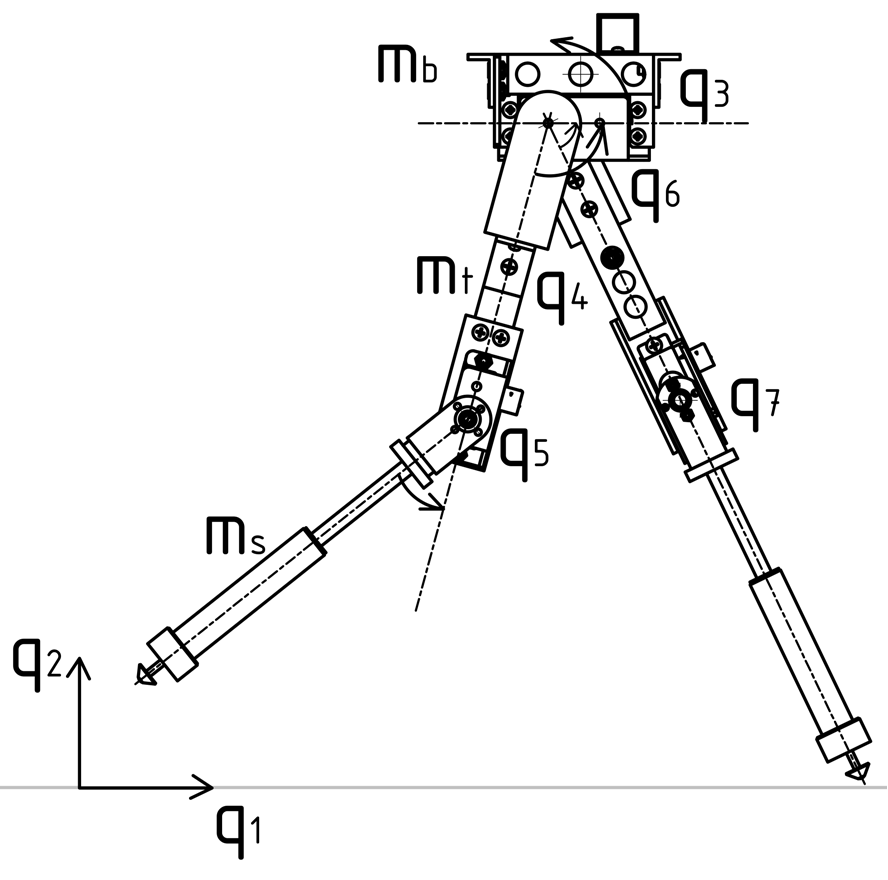
\includegraphics[width=0.8\linewidth]{jenafox/basic-coordinates/basic-coordinates.png}
            \caption{Degrees of freedom of the basic mechanical setup. The trunk (mass $m_b$) has three degrees of freedom ($q_1,~q_2,~q_3$), hip and knee of the right leg connect the thigh ($m_t$) to the body and shank ($m_s$) to the thigh respectively by one degree of freedom each ($q_4,~q_5$), the same counts for the left side ($q_6,~q_7$). (Adapted from~\cite{Renjewski2013}, p. 37)}%
            \label{fig:jenafox-dof}%
        \end{figure}
        % \noindent

        \begin{table}[H]
            \caption{Initial conditions used in the multi-body simulation consisting of the knee and hip angles of the swing leg,$~q_{5,~IC}$ and$~q_{4,~IC}$, the angle of the torso $q_{3,~IC}$ as well as their corresponding velocities $\dot{q}_{5,~IC},~\dot{q}_{4,~IC}$ and$~\dot{q}_{3,~IC}$. In addition,$~\gls{lambda}_{IC}$,~\ie the initial angle of~\gls{v}$_{\glsxtrshort{com}}$, was passed to the optimizer.} 
            \label{tab:initial-conditions}
            \begin{center}
                \begin{tabular}{ l|l|l|l }
                    \textbf{Initial conditions}     & \textbf{Description}                      & \textbf{Value}    & \textbf{Unit}                            \\ [0.5ex]
                    \hline \hline
                    $q_{5,~IC}$               & Angle of the right knee                   & $-29$             & $\left[\si{\degree}\right]$              \\
                    $q_{4,~IC}$               & Angle of the right hip                    & $-15$             & $\left[\si{\degree}\right]$              \\
                    $q_{3,~IC}$               & Angle of the torso                        & $15$              & $\left[\si{\degree}\right]$              \\
                    $\gls{lambda}_{IC}$                  & Angle of~\gls{v}$_{\glsxtrshort{com}}$    & $10$              & $\left[\si{\degree}\right]$              \\
                    $\dot{q}_{5,~IC}$         & Angular velocity of the right knee        & $0$               & $\left[\si{\radian\per\second}\right]$   \\
                    $\dot{q}_{4,~IC}$         & Angular velocity of the right hip         & $0$               & $\left[\si{\radian\per\second}\right]$   \\
                    $\dot{q}_{3,~IC}$         & Angular velocity of the torso             & $0$               & $\left[\si{\radian\per\second}\right]$   \\
                \end{tabular}
            \end{center}
        \end{table}
        % \noindent
        
        % where $\dot{q}_{5,~IC}$ and $\dot{q}_{4,~IC}$ are calculated from the initial velocity of the~\glsxtrshort{com} divided by the length of thigh and shank of the leg, respectively. 
        
        The used upper and lower bounds which were passed to the optimizer can be found in appendix~\ref{app:A}. The lower bounds are specifies as

        \begin{align}
            q_{i,~IC}~\geq~q_{i,~lb}~\forall~i,             \notag \\
            \dot{q}_{i,~IC}~\geq~\dot{q}_{i,~lb}~\forall~i, \notag \\
            \gls{lambda}_{IC}~\geq~\gls{lambda}_{lb},
            \label{eq:lower-bounds}%
        \end{align}
        % \noindent
        
        the upper bounds are specifies as

        \begin{align}
            q_{i,~IC}~\leq~q_{i,~ub}~\forall~i,             \notag \\
            \dot{q}_{i,~IC}~\leq~\dot{q}_{i,~ub}~\forall~i, \notag \\
            \gls{lambda}_{IC}~\leq~\gls{lambda}_{ub},
            \label{eq:upper-bounds}%
        \end{align}
        % \noindent
        
        where$~q_{i,~IC}$ and$~\dot{q}_{i,~IC}$ depict the initial conditions of each joint $i$ and~\gls{lambda}$_{IC}$ the initial angle of~\gls{v}$_{\glsxtrshort{com}}$.

        \subsection*{Objective Function}
        
        To ensure that the walking gait is periodic, the sum of absolute deviations between the initial and final state is used as the cost function. The states consist of$~\gls{q}$ and$~\dot{\gls{q}}$, with the absolute value of the torso angle to allow the frequency of the torso to be potentially half the frequency of a full step

        \begin{align}
            f &= \sum_{i = 3}^{7}~\lvert~q_i(\gls{t}_{end})~-~q_i(\gls{t}_0)~\rvert~+~\lvert~\dot{q}_i(\gls{t}_{end})~-~\dot{q}_i(\gls{t}_0)~\rvert
            \label{eq:objective-function}%
        \end{align}
        % \noindent

        where$~\gls{t}_0 = 0$ represents the initial state (\ie~\glsxtrshort{vlo}$_0$) and$~\gls{t}_{end}$ represents the final state (\ie~\glsxtrshort{vlo}$_1$). Further, the knee angle of the swing leg at touchdown$~q_{5,~TD}$ is included with an exponential penalty of the form 

        \begin{align}
            y &= -20 \cdot (0.6^{\vert x \vert} - 1)
            \label{eq:penalty}%
        \end{align}
        % \noindent
        
        which converges to a penalty value of 20, as can be seen in the following figure~\ref{fig:penalty}. Note that the knee is fully extended at$~q_{5,~TD} = 0\,\textrm{\si{\degree}}$. This ensures the smallest possible knee angle and thus the most extended leg possible at touchdown. 
        
        \begin{figure}[H]%
            \centering%
            \includestandalone{penalty/penalty}
            \caption{Exponential penalty of the knee angle of the swing leg at touchdown$~q_{5,~TD}$. Note that the knee is fully extended at$~q_{5,~TD} = 0\,\textrm{\si{\degree}}$. The penalty converges to a value of 20.}
            \label{fig:penalty}
        \end{figure}%
        % \noindent
        
        The same penalty was also applied to the final state of the hip and knee angles of the stance leg, to keep the angles as small as possible and thus to regain the upcoming~\glsxtrshort{vlo}$_1$ to the greatest possible extent again. Choosing an appropriate cost function is desirable to obtain smooth, well-behaved solutions and to ensure good convergence of the~\glsxtrshort{nlp}. Among others, the~\glsxtrshort{cot} is a widely used objective function, which, however, is difficult to optimize because the solutions tend to have discontinuities.~\cite{Kelly2017}
        
        % we will use the integral of the torque-squared cost function. This cost function tends to produce smooth, well-behaved solutions. This is desired for a few reasons. First, a smooth solution means that a piecewise polynomial spline will do a good job of approximating the solution, thus the nonlinear program will converge well. The second reason is that a smooth solution is easier to control on a real robotic system. Finally, minimizing the torque-squared tends to keep the solution away from large torques, which are sometimes undesirable in real robotic systems:
        
        % \begin{align}
        %     J &= \int\limits_{0}^{T} \left(\sum_{i = 1}^{5} u_{i}^2(\tau)\right) d\tau.
        % \end{align}
        % \noindent
        % %
        
        % There are many other cost functions that we could have used. One common function is~\glsxtrshort{cot}, which is a difficult cost function to optimize over, because the solutions tend to be discontinuous.

        \subsection*{Termination conditions}

        To increase the robustness of the model, possible error modes are identified in which the model shows unexpected or undesired behavior. The identified conditions are presented in table~\ref{tab:failure-modes}, such as the~\glsxtrshort{com} or one of the knees falling below a threshold in height, the robot starting to walk backwards as well as reaching a time or distance limit. If any of these cases occur, the simulation is aborted and the cost is penalized with a penalty function similar to the one used for the angles (see equation~\ref{eq:penalty}).
        
        \begin{table}[H]
            \caption{Identified failure modes of the system which may occur. A total of six failure modes were identified, the~\glsxtrfull{com} or one of the knees falling below a threshold in height, the robot starting to walk backwards as well as reaching a time or distance limit. If any of these cases occur, the simulation is aborted and the cost is penalized with a penalty function.} \label{tab:failure-modes}
            \begin{center}
                \begin{tabular}{ l|l }
                    \textbf{Failure Mode} & \textbf{Condition}                                                              \\ [0.5ex]
                    \hline \hline
                    Falling               & $\gls{y}_{\glsxtrshort{com}} \leq 0.15\,\textrm{\si{\metre}}$                      \\
                    Knee falling          & $\gls{y}_{knee_r},~\gls{y}_{knee_l} \leq 0.028\,\textrm{\si{\metre}}$                    \\
                    Walking backwards     & $\gls{v}_{\glsxtrshort{com}_x} \leq - 1\,\textrm{\si{\metre\per\second}}$  \\
                    Time limit            & $\gls{t}_{end} \geq 3.0\,\textrm{\si{\second}}$                                    \\
                    Distance limit        & $\gls{x}_{\glsxtrshort{com}} \geq 0.5\,\textrm{\si{\metre}}$
                \end{tabular}
            \end{center}
        \end{table}
    
        
%

\section{Summary}

In this chapter the individual steps, which are necessary to design a controller for the torso stabilization of a bipedal robot, are considered in detail. A MATLAB\textsuperscript{\textregistered} Simulink implementation of the JenaFox model was provided. The used neural network controller is based on the work of~\citeauthor{Geng2006}~\cite{Geng2006}. The initial and final conditions are defined by the~\glsxtrfull{vlo}. In order to be able to evaluate the individual iterations, a trajectory optimization problem was formulated in which the best solution is also the most periodic one,~\ie the solution in which the difference between the initial state (\glsxtrshort{vlo}$_0$) and final state (\glsxtrshort{vlo}$_1$) is as small as possible. Furthermore, termination conditions were identified to avoid undesired behavior.
